\documentclass{article}
\usepackage[T1]{fontenc}
\usepackage[utf8]{inputenc}
\usepackage{hyperref}
\usepackage{mathtools}
\usepackage{graphicx} 
\usepackage{titlesec}
\usepackage{float}
\usepackage{tabularx,booktabs,caption,ragged2e}
\usepackage{biblatex}
\usepackage{eurosym}
\usepackage{amsmath , amsfonts, amssymb}

\addbibresource{bibliographie.bib}
\setlength{\parindent}{0pt}
\captionsetup{skip=0.333\baselineskip}

\begin{document}

\tableofcontents
\section{Résumé}
\section{Introduction} 
Malgré l'augmentation du nombre de logements, les inégalités ne cessent d'aug-menter. D'après l'Insee le nombre de logements à presque doublé alors que la population n'a augmenté que 
de 37\%.\cite{evolution_hab}. La hausse des inégalités et la baisse du pouvoir d'achat étant au cœur de l'actualité. Lorsque en 2018, les dépenses de loyers pesaient 6.1\% dans l'IPC\cite{ipc_loyer} Nous avons trouvé bon de traiter la part des locataires en résidences principales. C'est à dire, la part des personnes vivant en résidence principale et qui n'en sont pas propriétaires. \\
Quels sont donc les facteurs influencent la part de locataire en résidence principale dans les départements Français? 

\section{Données utilisées}
L’une de nos première idée est de regarder du côté de l’âge. Nous avons donc pris deux premières variables explicatives qui sont respectivement : 
-la part des soixante-cinq-ans et plus
-la part des vingt-cinq ans et moins
On peut penser que les personnes plus âgées ayant travaillé toute leur vie on donc plus les moyens pour acheter leurs résidence principales que les jeunes de moins de vingt-cinq ans sortant pour certain tout juste de l’école.
L’école peut quant à lui aussi être un bon indicateur. En effet, on peut penser d’un point de vue macroéconomique, qu’une personne diplômée du supérieur gagne plus qu’une personne sans diplômes. Nous avons donc notre troisième variable explicative : 
-La part des diplômes supérieur ou égale au bac+5.
Ayant évoqué la richesse, il est intéressant d’essayer de trouver des variables explicatives du point de vue monétaire. C’est pourquoi nous avons décidé de prendre : 
-le taux de chômage 
-le taux de pauvreté 
Il est évident qu’on puisse s’attendre à une forte corrélation entre les deux, ce qui nous amènera par la suite à discuter de la multicolinéarité de notre modèle et choisir laquelle de ces variables nous allons retenir.
Par légèreté de pensée, on peut penser que les personnes investissant dans leurs résidence principale souhaitent avoir un certain confort autour d'elles. Comme par exemple la présence de commerce, d’école ou de proximité avec leur travail. Pour répondre à ce problème nous avons décidé de prendre comme sixième variable explicative :
-le taux d’urbanisation.
Enfin, notre dernière variable porte sur la part d’appartement. On peut penser que ces derniers étant plus petits et moins chers, certains investisseurs les préfèrent aux maisons afin de les mettre en location. De plus, pour les revenus les plus modestes, il est plus accessible d’accéder à une location d’appartement que de maison.
Tout d'abord, nous pouvons penser à plusieurs variables mais il faut bien prendre en compte que 
certaines ne 
soient pas disponibles au sein de l’insee. C’est pourquoi notre étude porte sur les départements de la France métropolitaine.
\newpage
\section{Modélisation}
\subsection{Premier modèle}
\subsubsection{Spécification du modèle}
Le premier modèle est formulé de la sorte : 
\begin{equation}
\begin{split}
		locataire_i =  \beta_1 &+ \beta_2dipsup_i + \beta_3jeune_i + \beta_4persagee_i \\
						&+ \beta_5appart_i + \beta_6chomage_i + \beta_7urba_i \\
						&+ \beta_8pauvrete_i + \varepsilon_i 
\end{split}
\end{equation}
\subsubsection{Interprétation des résultats }
On estime par la méthode des moindres carrés ordinaires les coefficients de l'équation précédente.
\begin{table}[H]
\centering
\caption{Première regression}
\begin{tabular}{l*{1}{cc}}
\toprule
Variable            & Coefficient         &  Écart-Type\\
\midrule
Constante & -10.84531 & 13.04414\\
dipsup	& 0,4028115	& 0,0844738\\
jeune  & 0,9092502 & 0,285378\\
persagee&  0,1280139 & 0,2338338\\
appart& 0,1638682 & 0,0307458\\
chomage& 0,1978747 & 0,2883803\\
ubra& 0,0080034 & 0,028728\\
pauvrete& 0,7533171& 0,1317305\\
\midrule
$N&          96         &            \\
SCE & $3873,9635$ \\
SCR & $485,248588$ \\
SCT & $4359,20494$ \\
\bottomrule
\end{tabular}
\end{table}
Le modèle s'écrit alors : 
\begin{equation*}
    \begin{split}
			\hat{locataire}_i = -10.85 &+ 0.40 \times dipsup_i + 0.91 \times jeune_i + 0.13 \times persagees_i \\
            &+ 0.16 \times appart_i + 0.2 \times chomage_i + 0.01 \times urba_i \\ 
			& + 0.75 \times pauvrete_i \\
    \end{split}
\end{equation*}
Le coefficient de détermination $R^{2}$ est calculé.
\begin{equation*}
    R^{2} = \frac{SCE}{SCT} = \frac{3873,9635}{4359,20494} = 0,8887
\end{equation*}
Ainsi que le coefficient de détermination ajusté aux nombres de variables.
\begin{equation*}
    \bar{R}^{2} = 1 - \frac{SCR/(N-K)}{SCT/(N-1)} = \frac{485,248588/88}{4359,20494/95} = 0,8798
\end{equation*}
Les deux coefficients sont élevés, cela laisse donc à supposer que l'ajustement de de la regression est de bonne qualité. Cependant, des tests de 
significativité (des paramètres et conjointe), et une étude de la multicolinéarité restent à être menés pour confirmer cela.
\subsubsection{Tests de significativité}
\label{sec:testSigni1}
Dans un premier temps, le test $F$ de significativité conjointe est fait. L'hypothèse nulle, et l'hypothèse alternative de ce test sont telles que :
\begin{equation*}
\begin{split}
    H_0 &: \beta_2 = \beta_3 = \dots \beta_K =0 \\
    H_1 &: \text{Au moins un }\beta_j \neq 0.
\end{split}
\end{equation*}
La statistique de test sous l'hypothèse nulle est distribuée selon une loi $F$ de Fisher.
\begin{equation*}
    F = \frac{SCE/(K-1)}{SCR/(N-K)} \sim F(K-1, N-K)
\end{equation*}
Pour un niveau de test à $\alpha = 5\%$, on compare la statistique calculée au quantile à $95\%$ de la distribution $F$ de Fisher avec 
comme degrés de liberté $7$ et $88$ respectivement au numérateur et au dénominateur. 
\begin{equation*}
    F_{1-\alpha} (K-1, N-K) = F_{0.95}(7, 88) = 2.121
\end{equation*}
Après calculs, $F = 100,364$. La statistique est supérieure au seuil, l'hypothèse nulle est rejetée au moins une variable permet d'expliquer le modèle.
\\ \\
Maintenant, il faut déterminer plus précisément quels sont les paramètres estimés significativement différents de 0. Pour cela, un test $t$ de 
significativité est effectué sur sur les $8$ paramètres :
\begin{equation*}
\begin{split}
    H_0 &: \beta_j =0 \\
    H_1 &: \beta_j \neq 0
\end{split}
\end{equation*}
La statistique de test calculée sous l'hypothèse nulle est distribuée selon une loi $t$ de Student : 
\begin{equation*}
    t_{\beta_j} = \frac{\hat{\beta_j}}{s_{\hat{\beta_j}}} \sim t(N-K)
\end{equation*}
Le niveau de test bilatéral est $\alpha = 5\%$ et la statistique en valeur absolue doit être comparée au quantile à $97,5\%$ de la distribution
 $t$ de Student à $88$ degrés de liberté, soit le seuil critique :
\begin{equation*}
    t_{1-\alpha/2}(N-K) = t_{0,975}(88) = 1,987289865 
\end{equation*}
Tous calculs faits, les résultats sont :
\begin{table}[H]
\centering
\caption{Statistique $t$}
\begin{tabular}{l*{1}{c}}
\toprule
Variable            &Statistique $t$\\
\midrule
constante      &   -.8314317\\
dipsup&    4.768476\\
jeune&    3.186125\\
persagee	 &5.329783\\
chomage&   -.6861589\\
urba   &    .2785922\\
pauvrete&    5.718624\\
\bottomrule
\end{tabular}
\end{table}
Les statistiques de test $t_{\beta_1},t_{\beta_7},t_{\beta_6}$ et $t_{\beta_3}$ sont inférieures en valeur en absolue au seuil. L'hypothèse nulle, est
acceptée pour ces paramètres, ils ne sont pas significatifs. Les variables $urba$, $chomage$ et $persagee$ seront donc retirées.

En revanche, $t_{\beta_2}, t_{\beta_3}, t_{\beta_5}, t_{\beta_8}$ sont supérieures en valeur absolue au seuil critique de $1,99$. On rejette l'hypothèse nulle pour ces paramètres
ils sont significatifs, les variables $dipsup$, $jeune$, $appart$ et $pauvrete$ permettent d'expliquer en partie $locataire$
\subsubsection{Etude de la multicolinéarité}
Une corrélation forte entre plusieurs variables explicatives peut induire une présence de multicolinéarité dans le modèle. Un calcul du VIF est fait pour chacune des variables.
\begin{table}[H]
\centering
\caption{Facteur d'inflation de la variance}
\begin{tabular}{l*{1}{c}}
\toprule
Variable            &         VIF\\
\midrule
constante & 0 \\
dipsup&    3,199862\\
jeune  &    12,48724\\
persagee	   &    14,58855\\
appart&    4,848903\\
chomage&    3,094149\\
urba   &    4,416773\\
pauvrete&    2,663816\\
\bottomrule
\end{tabular}
\end{table}
Il y a de la multicolinéarité dans le modèle, les variables $jeune$, $persagee$ et $appart$ ont un vif
élevé, elles seront donc retirées du modèle afin de traiter la multicolinéarité.
\subsection{Modèle final}
Un second modèle est formulé à la suite des résultats précédents. Ce modèle est tel que :
\begin{equation*}
    \begin{split}
            locataire_i =  \beta_1 &+ \beta_2dipsup_i + \beta_3jeune_i + \beta_5pauvrete_i + \varepsilon_i 
    \end{split}
\end{equation*}
Les paramètres du modèle sont estimés grace aux MCO.
\begin{table}[H]
\centering
\caption{}
\label{table:secondeReg}
\begin{tabular}{l*{1}{ccc}}
\toprule
Variable            & Coefficient&  Écart-type&Statistique t\\
\midrule
dipsup&    0,8001962&    0,0612541&    13,06355\\
jeune  &     0,960763&    0,1044884&    9,194929\\
pauvrete&    0,8518716&     0,096727&    8,806969\\
constante      &   -9,171721&    3,132582&   -2,927847\\
\midrule
$N$       &          96& SCE           &   3634,97216           \\
$R^{2}$ & 0,8339 & SCR & 724,232776   \\ 
$\bar{R}^2$ & 0,8284 & SCT & 4359,20494\\ 
\bottomrule
\end{tabular}
\end{table}
\subsubsection{Interprétation des résultats}
Les trois variables explicatives ont un effet positif sur la part de locataires en résidence principale. L'effet marginal de chaque variable peut être étudié, pour cela,
il suffit de dériver le modèle partiellement par rapport a une des variables pour connaître son effet marginal.
\begin{align*}
    &\frac{\partial locataire}{\partial dipsup} = \hat{\beta_2} \simeq 0,8 & &\frac{\partial locataire}{\partial jeune} = \hat{\beta_3} \simeq 0,96 & &\frac{\partial locataire}{\partial pauvrete} = \hat{\beta_3} \simeq 0,85
\end{align*}
Par exemple l'augmentation de la part de diplômés BAC+5 ou plus de 1 point entraînera une augmentation de la part de locataire de 0.8 points toutes choses étant égales par ailleurs.
L'effet le plus fort est l'effet de la population de moins de 25 ans, son effet marginal est presque un pour un. Ce résultat semble logique, puisque les populations jeunes sont très peu
propriétaires\cite{insee_portrait_social}.
\\
D'autre part, les personnes vivant sous le seuil de pauvreté sont moins enclin à acheter un bien immobilier, la location est donc privilégiée.
\\
En revanche, l'effet marginal de la part de hauts diplômés est surprenant. Il serait simple de penser que cet effet soit négatif, car une personne ayant fait de longues études aura un niveau
de vie supérieur à la moyenne et sera donc plus enclin à acheter un bien immobilier pour y vivre. Or ici, l'effet marginal est positif, la principale cause pourrait être le prix élevé de l'immobilier dans les grandes villes (lieu de travail des diplômés supérieurs) en particulier Paris\cite{prix_immo_paris}. Une autre cause pourrait être une mobilité accrue des diplômés
supérieurs comme les cadres. Ou bien une précarité grandissante des diplômés ne trouvant pas de travail\cite{precarite_etude_sup}
\\ \\
Les coefficients de détermination simple et ajusté sont relativement élevés, la qualité de l'ajustement du modèle est donc bonne. En théorie la
multicolinéarité a été traitée, pour confirmer cela, un calcul des VIF est effectué.
\begin{table}[H]
\centering
\caption{VIF}
\begin{tabular}{l*{1}{c}}
\toprule
Variable            &         VIF\\
\midrule
constante & 0 \\
dipsup & 1,18 \\
jeunes & 1,17 \\
pauvrete & 1,01 \\
\bottomrule
\end{tabular}
\end{table}
Les trois variables présentes dans le modèle ont un VIF proche de un, elles ne génèrent quasiment pas de multicolinéarité.
\subsubsection{Tests de significativité}
Des tests $t$ de significativité des paramètres sont fait pour déterminer si les paramètres estimés sont significatifs. Le test est le même que dans la
section 2.2.2. Les statistiques $t$ sont dans le tableau ~\ref{table:secondeReg}.
\\
Un niveau de test bilatéral de $\alpha = 5 \%$ est choisis, la statistique  $t$ doit donc être comparée au quantile à  $97,5\%$ de la distribution de
Student à 92 degrés de liberté. Le seuil critique est donc :
\begin{equation*}
t_{0,975}(92) = 1,986
\end{equation*}
Toutes les statistiques $t$ des paramètres de la regression sont supérieurs en valeur absolue au seuil critique. $H_0$ est rejetée dans tous les cas.
Tous les coefficients sont significativement différents de 0.
\\
La significativité est aussi testée avec le test $F$ de Fisher comme précédemment dans la section ~\ref{sec:testSigni1}. La statistique $F$ calculée est :
\begin{equation*}
    F =  \frac{3634,97216/3}{724,232776/92} = 153,918
\end{equation*}
Le niveau de test étant $5\%$, cette dernière est comparée au quantile à $95\%$ de la distribution de Fisher. Le seuil est donc :
\begin{equation*}
    F_{0,95}(3,92) = 2,704
\end{equation*}
Or $F > 2,704$ l'hypothèse nulle est rejetée, l'ajustement du modèle est de bonne qualité.
\subsubsection{Etude de la normalité des résidus}
Pour que les estimateurs soient de bonne qualité il faut que les erreurs de la régression suivent une loi normale pour cela les résidus sont sont calculés 
et trouvés dans la table ~\ref{tab:erreurs} des annexes. Ci dessous sont représentés les résidus sous forme d'histogramme, ainsi que, la courbe d'une 
loi normale de même espérance et variance $\mathcal{N}(0,2.76)$.
\begin{figure}[H]
	\centering
	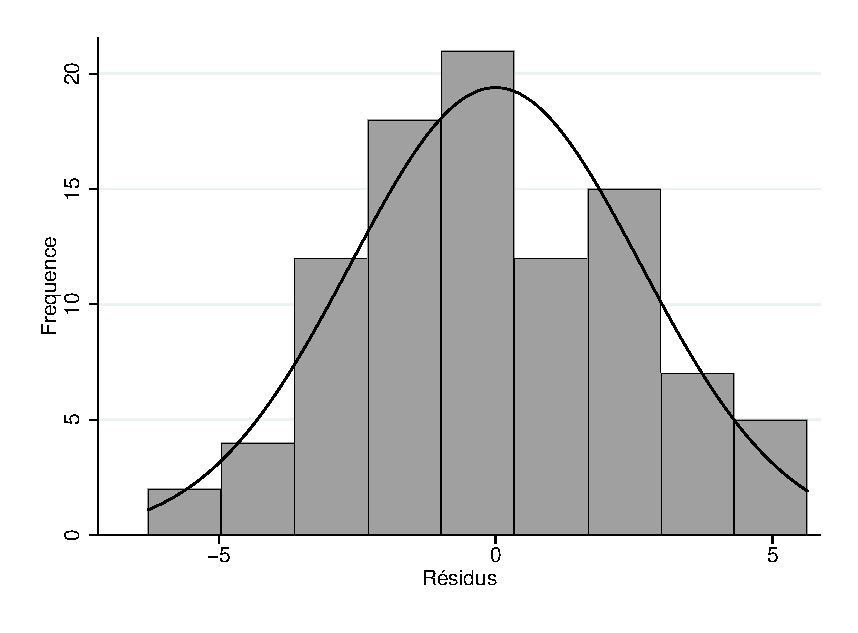
\includegraphics[scale=.6]{Graph.eps}
    \caption{Histogramme des erreurs}
	\label{fig:histogrammeErreur}
\end{figure}
Graphiquement, les résidus semblent suivre la distribution d'une loi normale de meme variance et espérance.
\subsubsection{Test sur l'hétéroscédasticité}
La présence d'hétéroscédasticité dans le modèle pourrait résulter en une mauvaise estimation de la variance des paramètres, dans ce cas là les tests
de significativité de ces paramètres deviendraient invalides. Le test de White d'hétéroscédasticité est réalisé. Les résidus au carré sont estimés par les MCO.
\begin{equation*}
    \begin{split}
        e^2_i = \phi_0 &+ \phi_1 dipsup_i + \phi_2 jeune_i + \phi_3 pauvrete_i\\
        &+ \phi_4 dipsup^2_i + \phi_5 jeune^2_i + \phi_6 pauvrete^2_i \\
        &+ \phi_7 dipsup_i \cdot jeune_i+ \phi_8 dipsup_i \cdot pauvrete_i + \phi_9 jeune_i \cdot pauvrete_i
    \end{split}
\end{equation*}
Les hypothèses sont :
\begin{align*}
    &H_0 : \phi_0 = \phi_1 = \dots =  \phi_9 = 0 & &\text{Homoscédasticité des erreurs} \\
    &H_1 : \text{Au moins un } \phi_j \neq 0 & &\text{Hétéroscédasticité des erreurs}
\end{align*}
La statistique de test est un multiplicateur de Lagrange : $\text{LM} = N \times R^2$ qui est comparé au quantile à $95\%$ (pour un niveau de test à $5\%$) 
de la distribution du khi-deux avec comme degrés de liberté $9$. Les résultats sont représentés dans le tableau ci dessous
\begin{table}[H]
\centering
\caption{Test de White}
\begin{tabular}{l*{1}{c}|{c}{c}}
    \toprule
    $N$ &          96 & $N \times R^2$ & 13,344\\
    $R^{2}$   &       0.139 & $\chi^2_{0.95}(9)$ &16,919 \\
    \bottomrule
\end{tabular}
\end{table}
La statistique de test est inférieure au seuil critique ($N \times R^2 < \chi^2(9)$). L'hypo-thèse nulle d'homoscédasticité est acceptée.
\\
Le modèle respecte donc bien toutes les hypothèses du modèle linéaire. Le modèle est bien spécifié et les estimateurs sont de bonne qualité.
\section{Conclusion}

dico : VIF = Variance inflation factor
MCO = moindres carrés ordinaires
\section{Bibliographie}
\printbibliography
\section{Annexes}
Matrice X
Première sortie
Matrice X finale
Sortie finale
Matrice e
Regression auxilière
\end{document}
